\documentclass[11pt,a4paper,titlepage]{article} 
\usepackage[utf8x]{inputenc} 
\usepackage[french]{babel} 
\usepackage[T1]{fontenc} 
\usepackage{amsmath} 
\usepackage{amsfonts} 
\usepackage{amssymb} 
\usepackage{graphicx} 
\usepackage[final]{pdfpages} 
\usepackage[toc,page]{appendix} 
\usepackage[top=2.5cm,bottom=2.5cm,right=2.5cm,left=2.5cm]{geometry} 
\usepackage{minted}
\author{SENE Victor } 
\title{Train-Simulation} 
\graphicspath{{img/}} 
\usepackage{fancyhdr} 
\pagestyle{fancy} 
\usepackage{lastpage} 
\renewcommand
\headrulewidth{1pt} 
\fancyhead[L]{Train-Simulation} 
\fancyhead[C]{Victor SENE} 
\fancyhead[R]{LO41 UTBM} 
\renewcommand
\footrulewidth{1pt} 
\fancyfoot[C]{\textbf{Page \thepage}} 
\fancyfoot[L]{Printemps 2016}

\newcommand{\HRule}{\rule{\linewidth}{0.5mm}}

\begin{document}

\begin{titlepage}
\begin{center}

% Upper part of the page. The '~' is needed because \\
% only works if a paragraph has started.


\textsc{\LARGE Université de technologie Belfort-Montbéliard}\\[1.5cm]

\textsc{\Large Système d’Exploitation : Principes et
	Communication  }\\[0.5cm]

% Title
\HRule \\[0.4cm]
{ \huge \bfseries LO41 - Simulation du fonctionnement d'un réseau ferroviaire\\[0.4cm] }

\HRule \\[1.5cm]
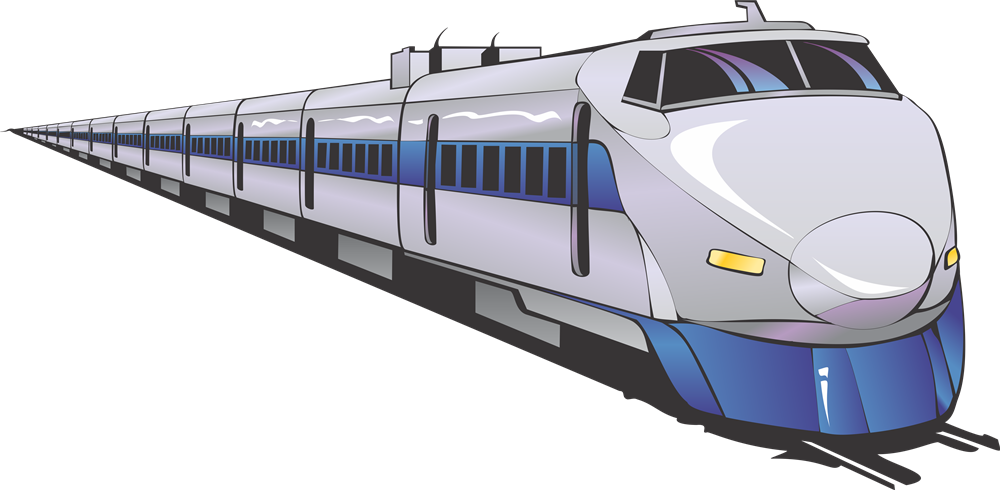
\includegraphics[width=1.0\textwidth]{./train.png}~\\[4cm]

% Author and supervisor
\begin{minipage}{0.4\textwidth}
\begin{flushleft} \large
\emph{Auteur:}\\
\textsc{Victor} SENE\\
\end{flushleft}
\end{minipage}
\begin{minipage}{0.4\textwidth}
\begin{flushright} \large
\emph{Professeur:} \\
Philippe \textsc{DESCAMPS}
\end{flushright}
\end{minipage}

\vfill

% Bottom of the page
{\large \today}

\end{center}
\end{titlepage}
%\tableofcontents
%\pagebreak
\newpage
\tableofcontents
\newpage

\section{Introduction}
Pour notre projet de LO41, nous avions pour but commun de modéliser le fonctionnement d'un réseau ferroviaire à partir d'algorithmes chargés de la coordination de l'ensemble des voies.
Dans notre sujet nous tiendrons compte des priorités que chaque train possède, de son sens de circulation ainsi que la capacité des voies. Ces contraintes permette de définir un ordre de déplacement et d'envisager des solutions pour éviter les collisions ou l'interblocage.

\section{Analyse du Sujet}
	\subsection{Sujet}
	Afin de modéliser le projet, j'ai décidé d'utiliser des threads pour représenter les trains du fait de la facilité d'implémentation de ceux-ci et de la cohérence avec le sujet. Dans un premier temps je voulais aussi faire en sorte que chaque voie soient un thread mais cela c'est révélé être un mauvais choix, donc je suis revenu simplement à des structures gérées par un aiguillage qui n'est qu'en fait une fonction autorisant ou non le déplacement et la réservation de voie.
	
	\subsection{Objectifs}
		\subsubsection{Objectifs fixés}
		\begin{itemize}
			\item L'objectif principal est d'éviter toute collision entre les trains en prenant en compte le sens de circulation
			\item Je voulais aussi pouvoir créer un grand nombre de train et que le programme puisse tourner sans problème.
			\item Je voulais perfectionner mon niveau en C et rendre un code aussi propre et cohérent que possible
			\item Pour finir, je souhaiterais éviter au maximum les problèmes de mémoire.
		\end{itemize}
		
		\subsubsection{Moyens mis en œuvre}
		\begin{itemize}
			\item Afin d'éviter les collisions j'ai inséré au sein de mes structures un indicatif de direction permettant aux trains de savoir si son sens de circulation est en adéquation avec celui de la voie.
			\item Afin de pouvoir gérer au mieux les problèmes d'interblocage j'ai décidé de réfléchir à un système de réservation des voies. Ainsi les trains ne pourraient circuler sur une voie que s'ils l'ont réservé auparavant. 
			Cette réservation donne des conditions supplémentaire à l'aiguillage centrale qui se doit d'interdire un passage sur une voie en cours de réservation ou en cours d'utilisation.
			\item En ce qui concerne le langage, j'ai utilisé la "caisse à outils" donné en cours et j'ai pu réfléchir à des problématiques de compilation lors de la création du MAKEFILE. Si je suis déçu de n'avoir pas eu plus d'occasions préalablement pour acquérir ce genre de connaissance, je suis satisfait d'avoir pu le faire maintenant et j'espère pouvoir retravailler avec ce langage. 
		\end{itemize}
		
		\subsubsection{La mémoire}
		À la fin du programme ou lors de son interruption volontaire, je libère la mémoire allouée pour les différents tableaux et je nettoie aussi les mutex et conditions pour les moniteurs des voies.

\section{Conception}

	\subsection{Réseau de pétri}
	Durant ma phase de conception, j'ai pu utiliser un des outils proposé en cours afin de modéliser le fonctionnement de certain point critique de la simulation.
	Voici un exemple de déplacement d'un TGV qui part de LIGNE et qui va vers la GARE:
	
	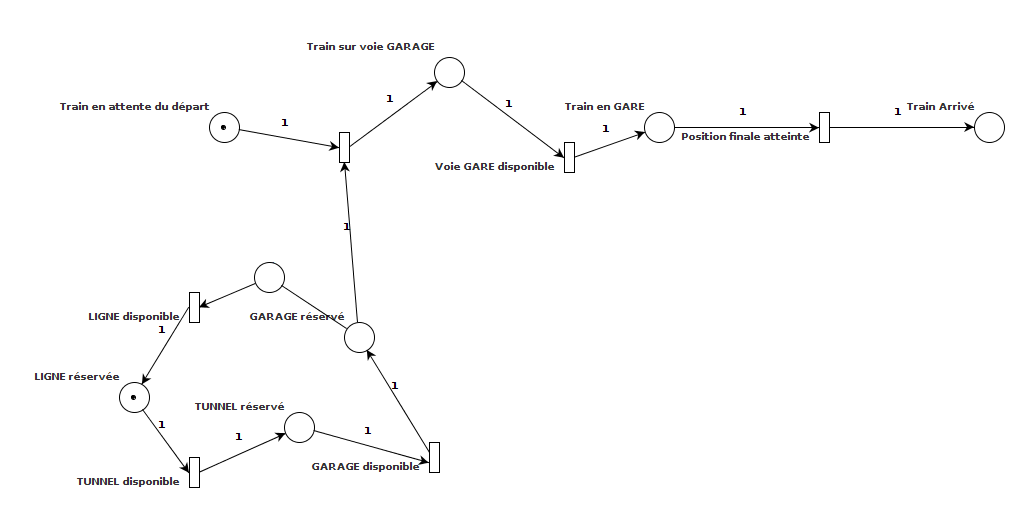
\includegraphics[width=1.0\textwidth]{./exPetri.png}~\\[0.1cm]
	\subsection{Système de Réservation}
	Le principal élément permettant d'éviter l'interblocage est le système de réservation. Alors pour cela j'utilise un booléen sur la voie et un tableau stockant les réservations en cours dans une structure de train. En pseudo-code le fonctionnement de la réservation serait ainsi :
	\begin{minted}{C}	
	TANT QUE on est pas sur un voie pour arreter le train
		SI la voie est pas reserve par moi 
		OU SI la voie est pleine 
		OU SI le sens courant de la voie ne me convient pas ALORS
			On reinitialise le tableau de reservation du train
			On attend que la voie soit libre
			On reprend la reservation de la position du train
		
		SINON 
			On reserve la voie
		FIN SI
		
		On va tester la reservation sur la voie suivante
	FIN TANT QUE
	\end{minted}
	\subsection{Structures}
		\subsubsection{Les voies}
		Pour circuler en train il préférable de le faire sur des voies prévues à cette effet. Si ici elle ne sont pas modéliser physiquement par l'intermédiaire d'un Thread ou d'un processus, les voies sont basées sur une même structures. Celles-ci sont créées et initialisées selon leurs spécificités au lancement du programme.
		
		La voie possède des attributs de réservation ($reserve, reserveId$)permettant de savoir si elle est actuellement en cours de réservation et si c'est le cas, quel train a réservé la voie.
		Un booléen $canStop$ indique si le train peut s'arrêter sur la voie en question.
		Chaque possède dans sa structure une condition permettant de faire attendre un train si la voie est occupée.
		Enfin chaque voie connait les voies qui lui sont directement adjacentes afin de pouvoir déterminer un enchainement de ligne formant le parcours du train.
		\begin{minted}{C}	
typedef struct struct_voie{
	int id;
	bool reserve;
	int reserveId;
	bool canStop;
	pthread_cond_t voieLibre;
	
	int nbTrainAct;
	int nbMaxTrain;
	int nbVoieLeft;
	int nbVoieRight;
	struct struct_voie** voieLeft;
	struct struct_voie** voieRight;
	
	int currentSens;
	int sens;
		//  -1 = vers la gauche
		//  0 = dans les 2 sens
		//  1 = vers la droite
	
	int typeTrain[3];
		//  [0] = autorise TGV
		//  [1] = autorise GL
		//  [2] = autorise M
}Voie;	
		\end{minted}
		\subsubsection{Les trains}
		Chaque train étant un thread il faut cependant une structure pour permettant par exemple de connaitre la position de celui-ci, son sens de circulation et sa priorité.
		Un tableau de réservation permet de lister les réservations faites et de les effacer rapidement en cas d'échec à la réservation d'un enchainement de voies.
		On pourra se simplifier la vie en déclarant un $enum$ pour les priorités.
		\begin{minted}{C}
typedef struct {
	int id;
	int sens;
		//  -1  = vers la gauche
		//   1  = vers la droite
	int priorite;
		//  [0] = TGV
		//  [1] = GL
		//  [2] = M
	Voie* position;
	Voie* startPos;
	Voie* endPos;
	Voie** reservationTab;
	int nbReservation;
}Train;
		\end{minted}
		Lors de la création d'un train j'utilise une fonction d'initialisation permettant de choisir dynamiquement le sens et la priorité de circulation. Mais chaque thread se voit priorisé au sein même de sa structure. Je définis donc les attributs du Thread pour que les threads TGV soient prioritaires sur les Marchandises par exemple. L'algorithme d'ordonnancement des threads est modifié et j'utilise un FIFO.
		\begin{minted}{C}
pthread_attr_t ordonnancement(pthread_attr_t tattr, struct sched_param param, int priority){
	// Initialisation avec attributs par defaut
	pthread_attr_init(&tattr);
	// Sauvegarde des parametres actuels
	pthread_attr_getschedparam (&tattr, &param);
	// Changement politique ordonnancement
	pthread_attr_setschedpolicy(&tattr, SCHED_FIFO);
	// Changement priorite
	param.sched_priority = priority;
	// Application nouveau parametres
	pthread_attr_setschedparam(&tattr, &param);
	
	return tattr;
}
		\end{minted}	
	\subsection{Constantes \& Variables globales}
	J'utilise des constantes globales pour pouvoir faire éventuellement évolué le réseau ferré.
	\begin{minted}{C}
#define NB_VOIE 13
#define NB_AIGUILLAGE 4
#define MAX_TRAIN 10000000
#define TGV_PRIORITY 100
#define GL_PRIORITY 50
#define M_PRIORITY 10

int nbTrain; //nombre totale de train
int nbTGV, nbGL, nbM;
Voie* tabVoie; //tableau de l'ensemble des voies
pthread_mutex_t mutex; //mutex principal
pthread_t* tid; //tableau de threads pour les trains
	\end{minted}
	
	\subsection{Paramètres}
	Pour introduire un peu de modularité, j'ai décidé de proposer à l'utilisateur de choisir au lancement combien de trains et de quel type il en veut. Cependant le réseau ferré reste le même.
	\begin{minted}{C}
if (argc == 1) {
	nbTGV = 1000;
	nbGL = 1000;
	nbM = 1000;
}
	else{
	nbTGV = atoi(argv[1]);
	nbGL = atoi(argv[2]);
	nbM = atoi(argv[3]);
}
nbTrain = nbTGV + nbGL + nbM;
	\end{minted}
	\subsection{Makefile}
	N'ayant que peu de connaissance en ce qui concerne la compilation, j'ai réalisé un makefile pour faciliter la compilation et les tests. J'ai essayé de le faire le plus modulaire possible afin de pouvoir le réutiliser. J'ai défini trois méthodes :
	\begin{itemize}
		\item $all$ qui compile l'ensemble du projet en créant les $.c$ à partir des $.o$ avec le concours des bibliothèques nécessaires pour les threads notamment.
		\item $clean$ qui efface les $.o$ et l'exécutable.
		\item $run$ qui réutilise $clean$ pour nettoyer les binaires, compiler l'ensemble du projet et l'exécuter avec les paramètres par défauts.
	\end{itemize}
\section{Conclusion}
	\subsection{Améliorations possibles}
	Plusieurs améliorations sont possibles notamment au niveau de la définition des voies qui est dans mon cas très séquentielle et manque clairement de modularité. J'ai décidé de définir les voies de cette manière car au début cela me paraissait plus clair. Cependant lors de l'implémentation et de l'évolution je me suis vite rendu compte que c'était compliqué à maintenir.
	Afin de rendre le projet plus lisible et agréable, je pense qu'il serait préférable d'améliorer l'affichage. J'ai d'ailleurs commencé à le faire mais l'ensemble n'est pas totalement fonctionnel ne me permettant de vous le présenter.
	\subsection{Bilan}
	Dans ce projet, j'ai été ravi de pouvoir faire usage du C car ma formation ne m'a pas encore permis d'en faire énormément. De plus l'imaginaire du projet était amusant et motivant car réaliste.
	Le fait d'avoir pu appliquer les connaissances acquises en cours était un but et une source de motivation. Je suis un petit peu déçu de pas avoir connu le sujet plus tôt ce qui m'aurait permis d'y réfléchir en amont. 
	Malgré les nombreuses difficultés rencontrées du fait de mon bagage en C qui est assez pauvre, j'ai apprécié ce projet et cette unité de valeur.



\end{document}